%%%%%%%%%%%%%%%%%%%%%%%%%%%%%%%%%%%%%%%%%
% Based on template downloaded from:
% http://www.LaTeXTemplates.com
%
% Original author:
% Linux and Unix Users Group at Virginia Tech Wiki 
% (https://vtluug.org/wiki/Example_LaTeX_chem_lab_report)
%
% License:
% CC BY-NC-SA 3.0 (http://creativecommons.org/licenses/by-nc-sa/3.0/)
%
%%%%%%%%%%%%%%%%%%%%%%%%%%%%%%%%%%%%%%%%%
\documentclass{article}

\usepackage[version=3]{mhchem} % Package for chemical equation typesetting
\usepackage{siunitx} % Provides the \SI{}{} and \si{} command for typesetting SI units
\usepackage{graphicx} % Required for the inclusion of images
\usepackage{natbib} % Required to change bibliography style to APA
\usepackage{amsmath} % Required for some math elements 
\usepackage{listings}
\usepackage{xcolor}


\definecolor{codegreen}{rgb}{0,0.6,0}
\definecolor{codegray}{rgb}{0.5,0.5,0.5}
\definecolor{codepurple}{rgb}{0.58,0,0.82}
\definecolor{backcolour}{rgb}{0.95,0.95,0.92}

\lstdefinestyle{mystyle}{
    backgroundcolor=\color{backcolour},   
    commentstyle=\color{codegreen},
    keywordstyle=\color{magenta},
    numberstyle=\tiny\color{codegray},
    stringstyle=\color{codepurple},
    basicstyle=\ttfamily\footnotesize,
    breakatwhitespace=false,         
    breaklines=true,                 
    captionpos=b,                    
    keepspaces=true,                 
    numbers=left,                    
    numbersep=5pt,                  
    showspaces=false,                
    showstringspaces=false,
    showtabs=false,                  
    tabsize=2
}

\lstset{style=mystyle}

\setlength\parindent{0pt} % Removes all indentation from paragraphs

\renewcommand{\labelenumi}{\alph{enumi}.} % Make numbering in the enumerate environment by letter rather than number (e.g. section 6)

%\usepackage{times} % Uncomment to use the Times New Roman font

%----------------------------------------------------------------------------------------
%	DOCUMENT INFORMATION
%----------------------------------------------------------------------------------------

\title{\textbf{REMODEL automated report} \\ A Community Poll on Reproducibility in Computational Geosciences} % Title

\author{Robert \textsc{Reinecke}} % Author name

\begin{document}

\maketitle % Insert the title, author and date

\begin{center}
\begin{tabular}{l r}
Report last updated: & 19th May, 2021\\
Compilation date: & \today
\end{tabular}
\end{center}

This document summerizes a full analysis for detailed results. \textbf{It is not a full publication but rather an automated representation of the data present in this repository}

It summarizes the extensive results and builds the foundation for the publication of a journal paper.
It will also be distributed along with the data in the course of a journal and data publication.

\section{Aim of this survey}
Software development has become an integral part of the geosciences$^{1}$ as models and data processing get more sophisticated.
Paradoxically, it poses a threat to scientific progress as the pillar of science, reproducibility, is seldomly reached$^{2}$.
Software code tends to be either poorly written and documented or not shared at all; proper software licenses are rarely attributed.
This is especially worrisome as scientific results have potential controversial implications for stakeholders and policymakers and may influence the public opinion for a long time$^{3}$.

In recent years, progress towards open science has led to more publishers demanding access to data and source code alongside peer-reviewed manuscripts4,5. Still, recent studies find that results can rarely be reproduced $^{6,7}$.

In this project, we conduct a poll among the geoscience community which is advertised via scientific blogs (AGU, EGU), research networks (researchgate.net and mailing lists), and social media.
Therein, we strive to investigate the causes for that lack of reproducibility.
We take a peek behind the curtain and unveil how the community develops and maintains complex code and what that entails for reproducibility$^{8}$ .
Our survey includes background knowledge, community opinion, and behaviour practices regarding reproducible software development.

We postulate that this lack of reproducibility$^{9}$  might be rooted in insufficient reward within the scientific community, insecurity regarding proper licencing of software and other parts of the research compendium as well as scientists’ unawareness about how to make software available in a way that allows for proper attribution of their work.
We question putative causes such as unclear guidelines of research institutions or that software has been developed over decades$^{10}$ , by researchers' cohorts without a proper software engineering process¹ and transparent licensing.

To this end, we also summarize solutions like the adaption of modern project management methods from the computer engineering community$^{11}$  that will eventually reduce costs while increasing the reproducibility of scientific research$^{8}$ .

1 A comment to "Most Computational Hydrology is not Reproducible, so is it Really Science?” R.W. Hut, N.C. van de Giesen, N. Drost, Water Resources Research, 2017\\
2 Hutton, C., Wagener, T., Freer, J., Han, D., Du\_y, C., and Arheimer, B., Most computational hydrology is not reproducible, so is it really science? Water Resources Research, 2016\\
3 Munafò, M., Nosek, B., Bishop, D. et al., A manifesto for reproducible science. Nat Hum Behav, 2017\\
4 Executive editors, G. Editorial: The publication of geoscientifc model developments v1.2. Geoscientifc Model Development, 2019\\
5 Katz, D. S., Niemeyer, K. E., and Smith, A. M., Publish your software: Introducing the journal of open source software (joss), Computing in Science Engineering, 2018\\
6 Stagge, J. H., Rosenberg, D. E., Abdallah, A. M., Akbar, H., Attallah, N. A., and James, R., Assessing data availability and research reproducibility in hydrology and water resources. Scientific data, 2019\\
7 Añel, J. A., García-Rodríguez, M., and Rodeiro, J.: Current status on the need for improved accessibility to climate models code, Geosci. Model Dev., 2021\\
8 Stodden, V., The reproducible research standard: Reducing legal barriers to scientific knowledge and innovation. IEEE Computing in Science \& Engineering, 2009\\
9 https://www.nature.com/news/1-500-scientists-lift-the-lid-on-reproducibility-1.19970\\
10 Muller, C., Schaphoff, S., von Bloh, W., Thonicke, K., and Gerten, D., Going open-source with a model dinosaur and establishing model evaluation standards. EGU, 2018\\
11 https://software.rajivprab.com/2019/11/25/the-birth-of-legacy-software-how-change-aversion-feeds-on-itself\\


Our larger questions:
\begin{itemize}
	\item Is eproducibility is an issue in the geosciences? Are bad code and documentation the root cause of that issue?
	\item Is model software too complex? Does that hinder reproducibility?
	\item Are researchers missing the tools and know-how (methods, licenses etc.) to build good model code?
	\item Is missing funding and missing time preventing researchers from making their models more accessible?
\end{itemize}

We define reproducibility as:

"Reproducibility in the context of modeling in the geosciences means that results obtained by a modeling experiment should be achieved again with a high degree of agreement when the study is replicated with the same model design, inputs, and general methodology by different researchers.

We explicitly exclude the retracing of results by means of using a different modeling environment (including variations in model concept, algorithms, input data or methodology)."

\section{Data processing}
We designed the survey according to standards from psychology research. We apply descriptive statistics to analyse demographic background and basic analysis.
Further, we apply inferential statistical methods to test the unerlying hypotheses.

The raw data of the survey is stored in the folder \textbf{LiveData}. \textbf{The raw data has not been modified or cleaned in any way.}
To run some basic cleanup run the follwoing script: 

\begin{lstlisting}[language=Python]
import process_data.py as p
p.process()
\end{lstlisting}

\section{Results}
All data processing and plotting (including building this document) can be executed by running \lstinline{python run.py}.
Plotting details and addtional processing can be found in th script \lstinline{plot_all.py}.

Our main hypothesis for this analysis where the following:
\begin{itemize}
	\item \textbf{H1} Young scientists develop software more actively than established researchers.
	\item \textbf{H2} Young scientists are more familiar with software licenses than established researchers. 
	\item \textbf{H3} Young scientists are more familiar with modern development methods than established researchers. 
	\item \textbf{H4} Senior researcher percieve reproducability as a lesser problem than early career researchers.
 	\item \textbf{H5} Software complexity is the main reason for a lack of reproducability.
 	\item \textbf{H6} Researchers code frequently but without knowledge about proper engineering methods, licences and tools. 
 	\item \textbf{H7} The most frequently used language is still C/Fortran. Younger scientists tend to use Python and R; this is consistent throughout fields 
 	\item \textbf{H8} Most researchers are autodidacts when it comes to coding. 
 	\item \textbf{H9} Most researchers have never reproduced code with the original model. Only with their own model. This differs between fields. 
 	\item \textbf{H10} Practitioners and researchers perceive the issue of reproducibility differently. Scientists are more aware (?). 
	\item \textbf{H11} There are more researchers that apply software than they are ones that develop it. This differs between activities and fields. 
 	\item \textbf{H12} Most researcher do not know if their software belongs to them. 
 	\item \textbf{H13} Models that are available are hard to use. Causes?: Bad code, no documentation, no input data 
 	\item \textbf{H14} Senior researchers are convinced their work is reproducible. (much more at least than young scientists) 
 	\item \textbf{H15} The smaller the scale the more reproducible and accessible. 
 	\item \textbf{H16} Researchers think that their software is bug free and always correspond to their intended implementation. 
 	\item \textbf{H17} Most senior scientists think investment in FOSS doesn’t pay off. 
 	\item \textbf{H18} Senior researchers think that their code/project is easier to understand but that conflicts with reality. And younger researchers have the opposite understanding. 
 	\item \textbf{H19} We need more funding to enable reproducible computational science. 
 	\item \textbf{H20} New research software tends to be FOSS, big players are often legacy software grown over decades which is hard to reimplement as FOSS. 
\end{itemize}

\subsection{Sample Characteristics (demographics)}
Who were our participants?
Here we present characteristics of the participants in our poll, i.e. their current career stage, their years of research experience, their geo-scientific field and scale as well as their current focus of work.
This is purely descriptive statistics.
As we welcomed everyone to our poll, we did not form any assumptions regarding sample characteristics.
Also, we tried, but might not have reached a representative sample of the population of geo-scientists.

Here, we report basic sample characteristics. Also, we can check for and report any salient sample properties.

Corresponding survey questions:

\begin{itemize}
	\item DM01 - What career stage are you in?
	\item DM02 - For how long have you been working in your research field?
	\item DM06 - To which field within the geosciences does your research mainly belong?
	\item DM05 - What geographic scale are you working on?
	\item DM07 - What is the focus of your work?
\end{itemize}

\begin{figure}[!p]
    \centering
    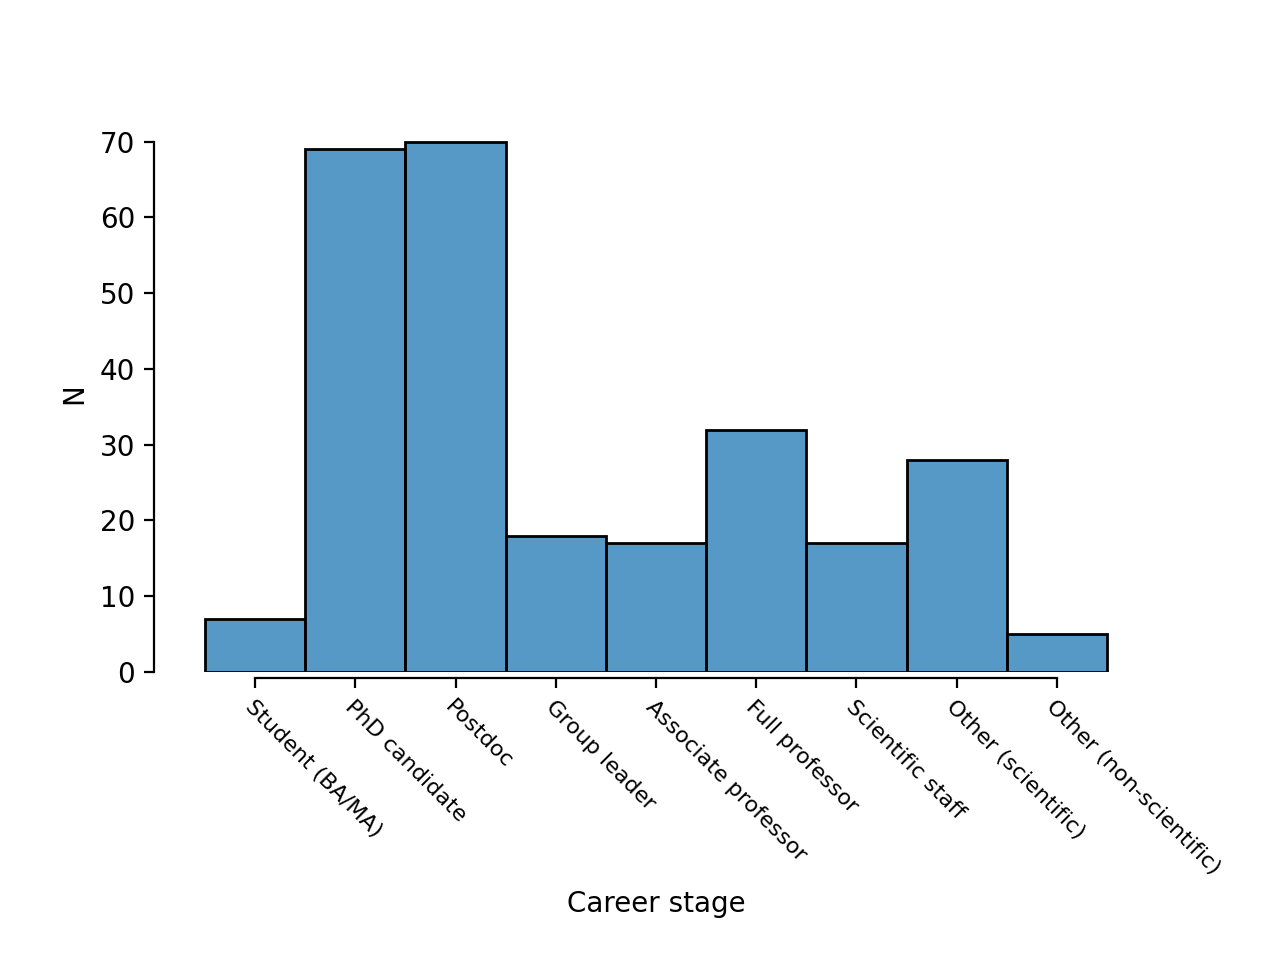
\includegraphics[width=\textwidth]{../figs/DM01.png}
	\caption{DM01 - Career stage of participants}
    \label{fig:dm01}
\end{figure}

\begin{figure}[!p]
    \centering
    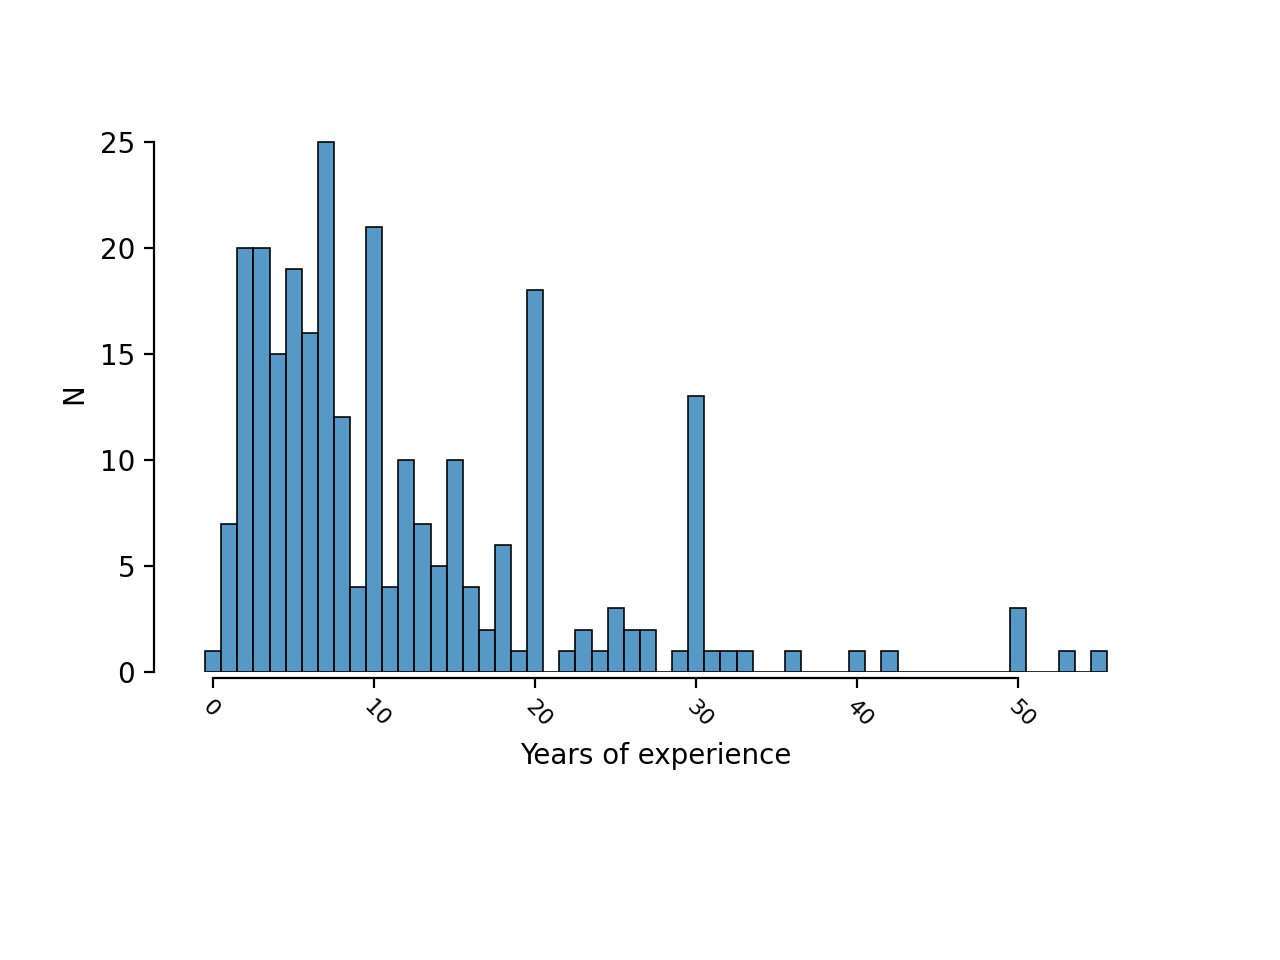
\includegraphics[width=\textwidth]{../figs/DM02_01.png}
	\caption{DM02 - For how long have you been working in your field?}
    \label{fig:dm02}
\end{figure}

\begin{figure}[!p]
    \centering
    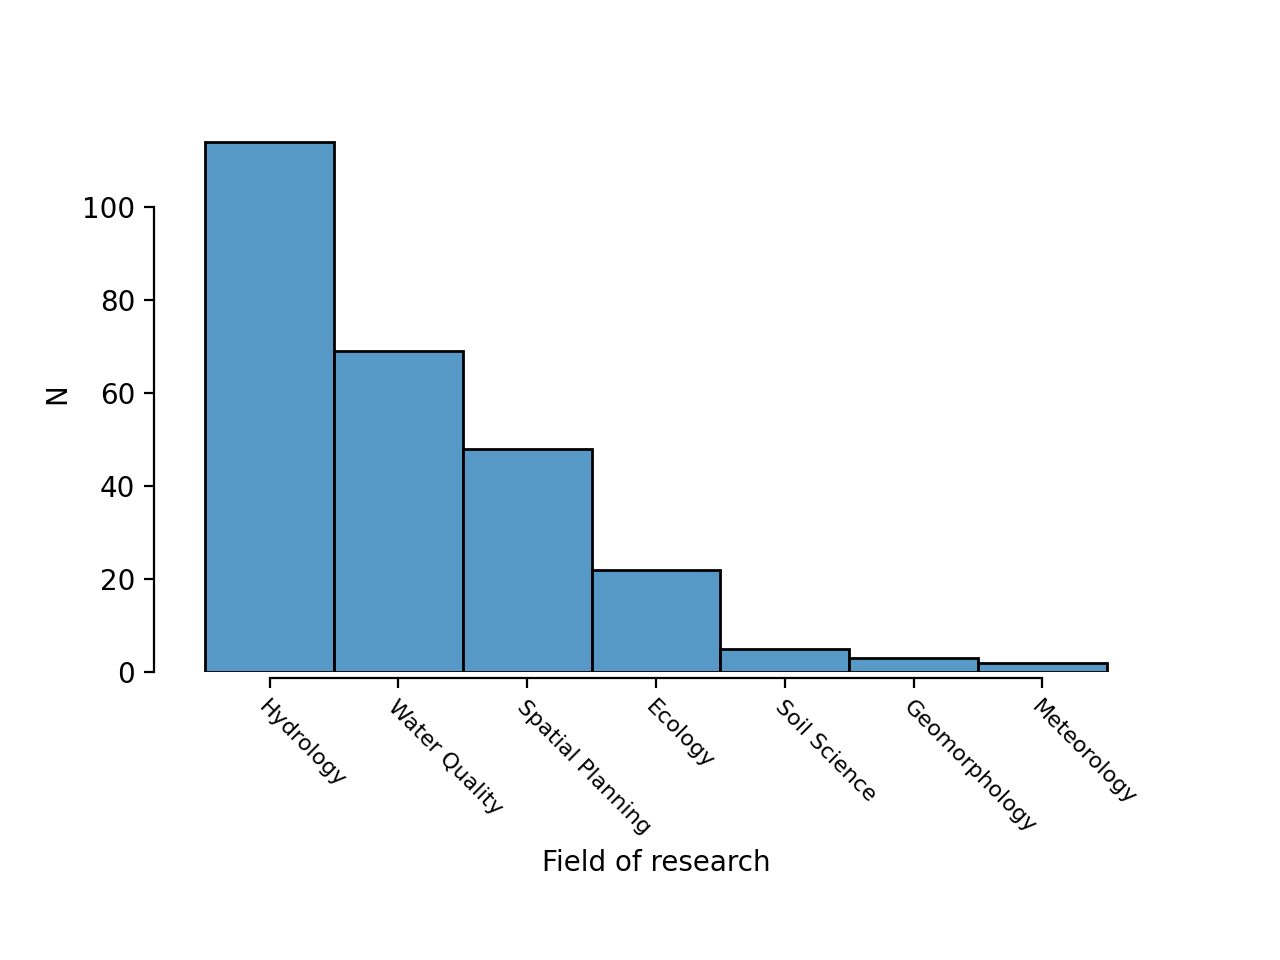
\includegraphics[width=\textwidth]{../figs/DM06.png}
	\caption{DM06 - Which field do you belong to?}
    \label{fig:dm06}
\end{figure}

\begin{figure}[!p]
    \centering
    \includegraphics[width=\textwidth]{../figs/DM05.png}
	\caption{DM05 - What scale are you working on?}
    \label{fig:dm05}
\end{figure}

\begin{figure}[!p]
    \centering
    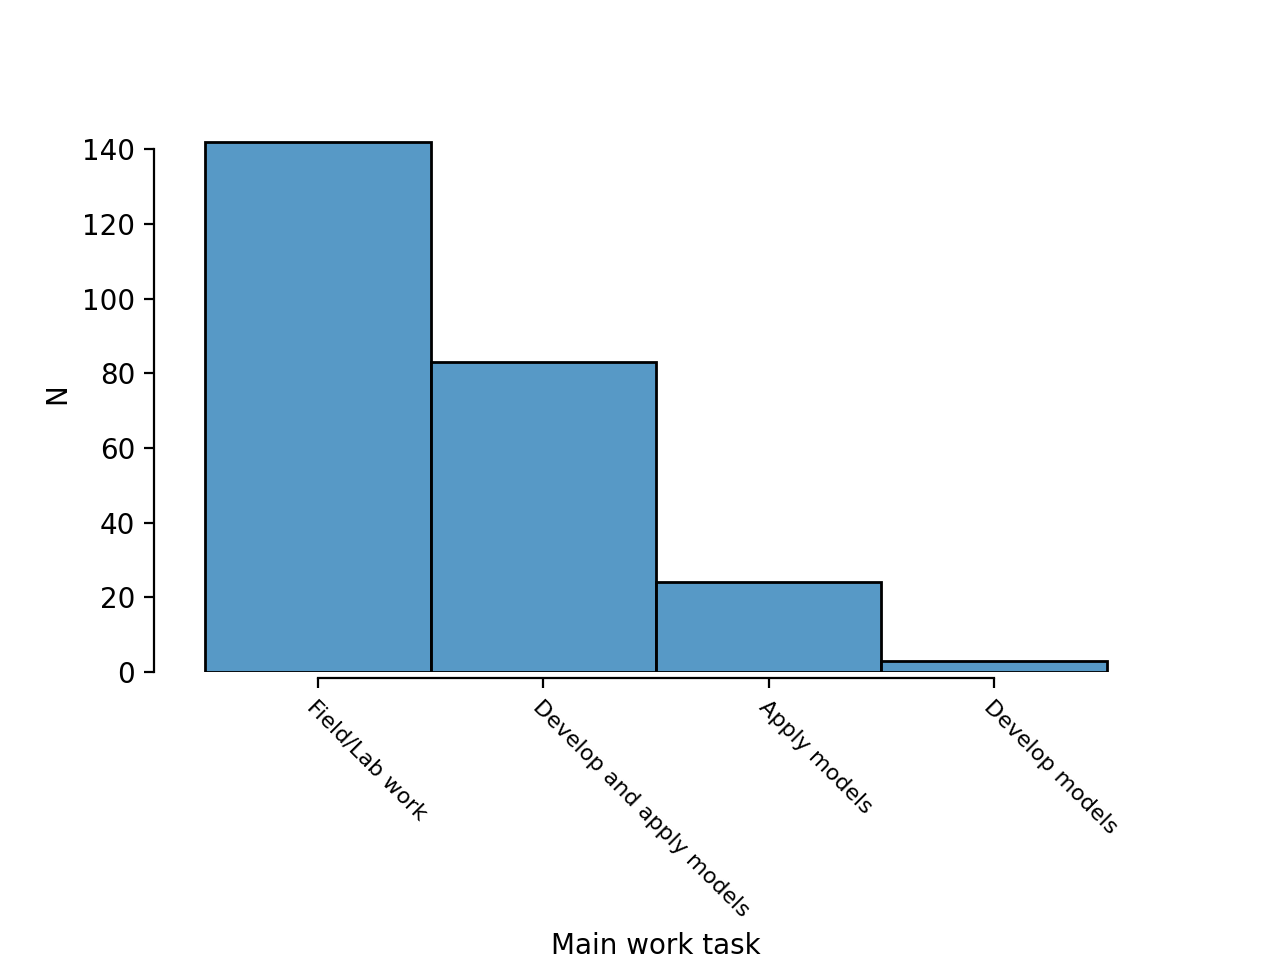
\includegraphics[width=\textwidth]{../figs/DM07.png}
	\caption{DM07 What is the focus of your work?}
    \label{fig:dm07}
\end{figure}
\newpage

\subsection{Community Opinion on Reproducibility}
This part covers people's view and opinion.
We assume that our defintion of reproducibility was used (annotated at several points in the poll).

Analysis Steps:
\begin{itemize}
	\item plot corresponding questions (across full sample)
	\item perform statistical testing of our above stated hypotheses (across subgroups, e.g. early career vs senior researcher)
	\item perform further data exploration (NOT hypothesis testing) - this might inspire future research, e.g. correlation analysis
\end{itemize}
 
Corresponding survey questions:
\begin{itemize}
	\item O101 - How strongly do you agree with the following statements?
	\item O103 - What are the reasons for a lack of reproducibility?
	\item S113 - How long do you think does it take for an average PhD student to efficiently work with your research software?
\end{itemize}

Corresponding hypotheses
\begin{itemize}
	\item H4 Senior researcher percieve reproducability as a lesser problem than early career researchers.
 	\item H5 Software complexity is the main reason for a lack of reproducability.
	\item H10 Practitioners and researchers perceive the issue of reproducibility differently. Scientists are more aware (?).
	\item H13 Models that are available are hard to use. Causes?: Bad code, no documentation, no input data.
	\item H14 Senior researchers are convinced their work is reproducible. (much more at least than young scientists).
	\item H16 Researchers think that their software is bug free and always correspond to their intended implementation.
\end{itemize}

O101: Opinion on Reproducibility in Geo-Sciences: How strongly did participants generally agree with statements?
Do they consider it a problem at all? Do they think that their work is reproducible?

\begin{figure}[!p]
    \centering
    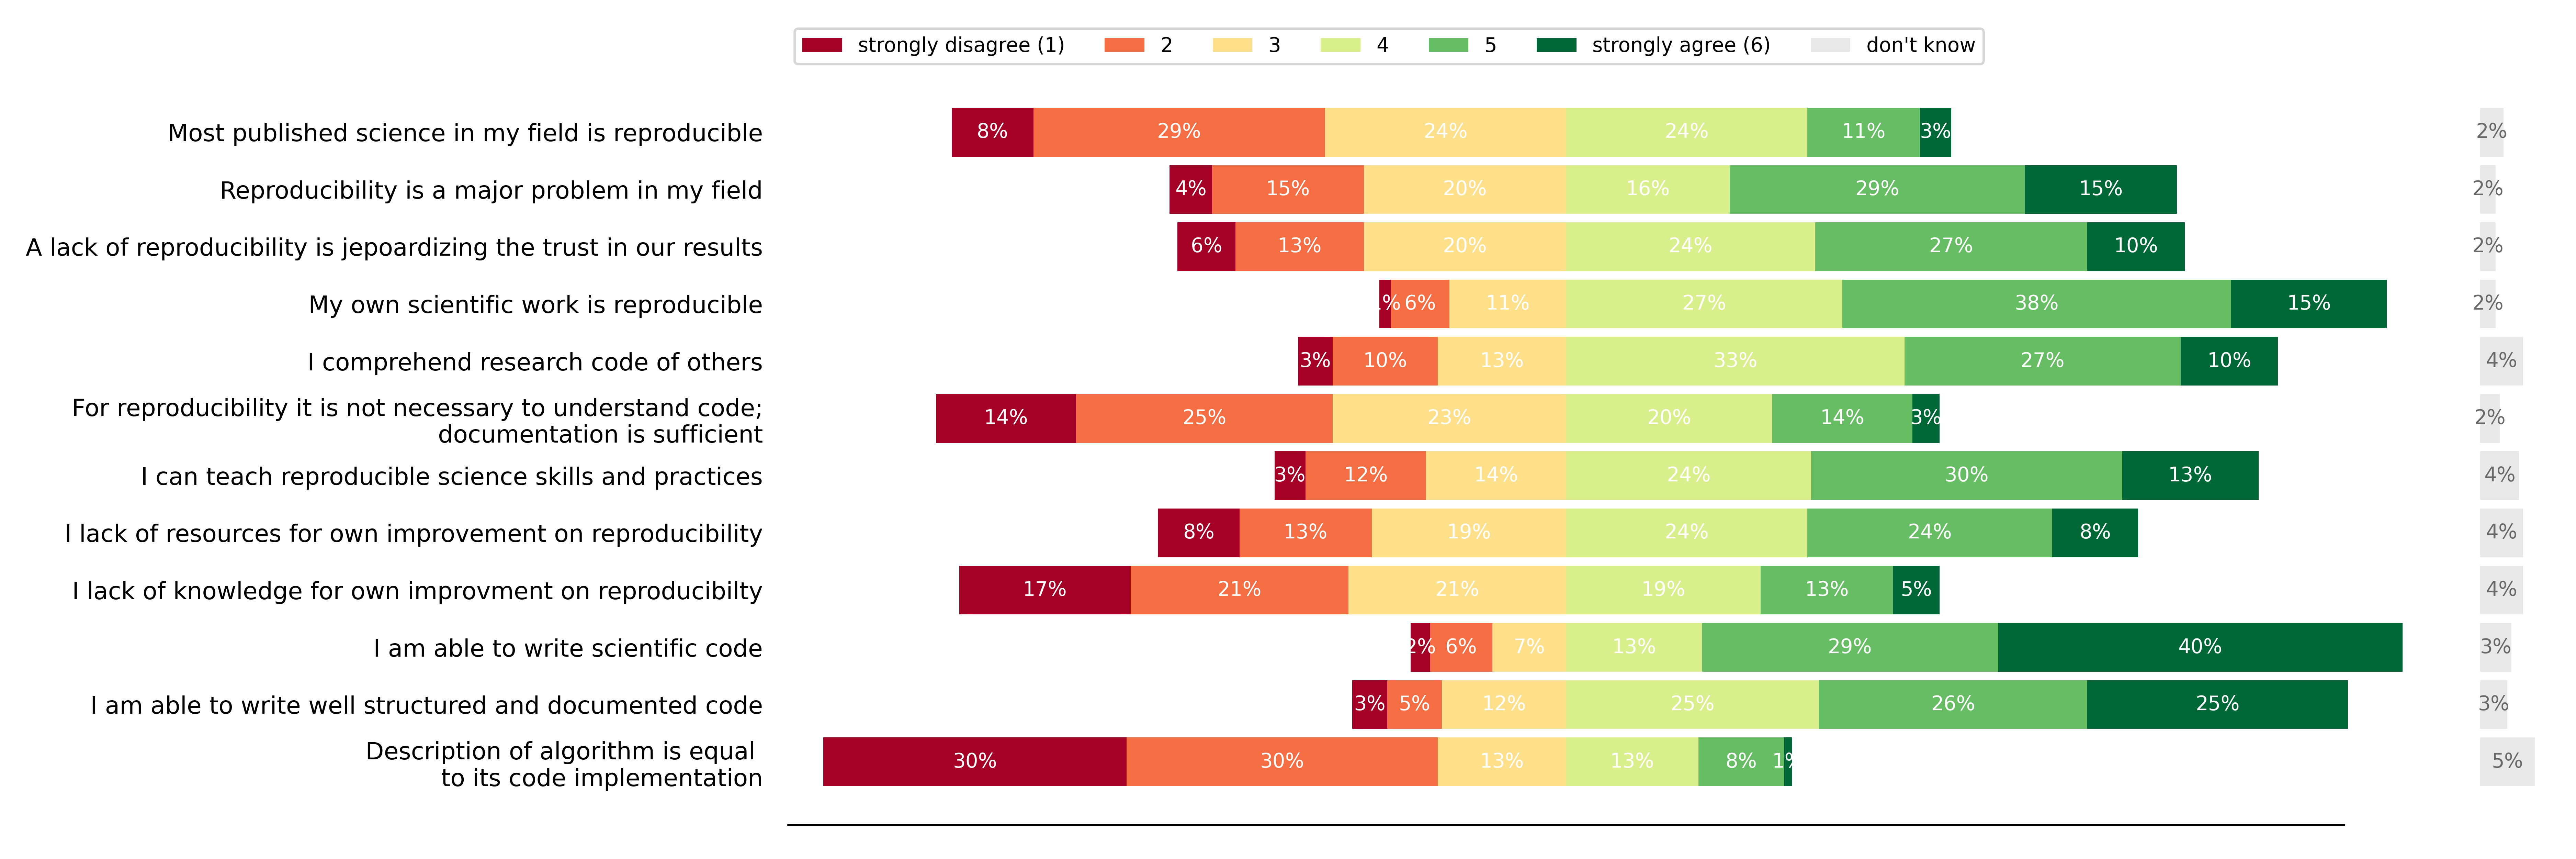
\includegraphics[width=\textwidth]{../figs/O101.png}
	\caption{O101 How strongly do you agree with the following questions?}
    \label{fig:O101}
\end{figure}

\begin{figure}[!p]
    \centering
    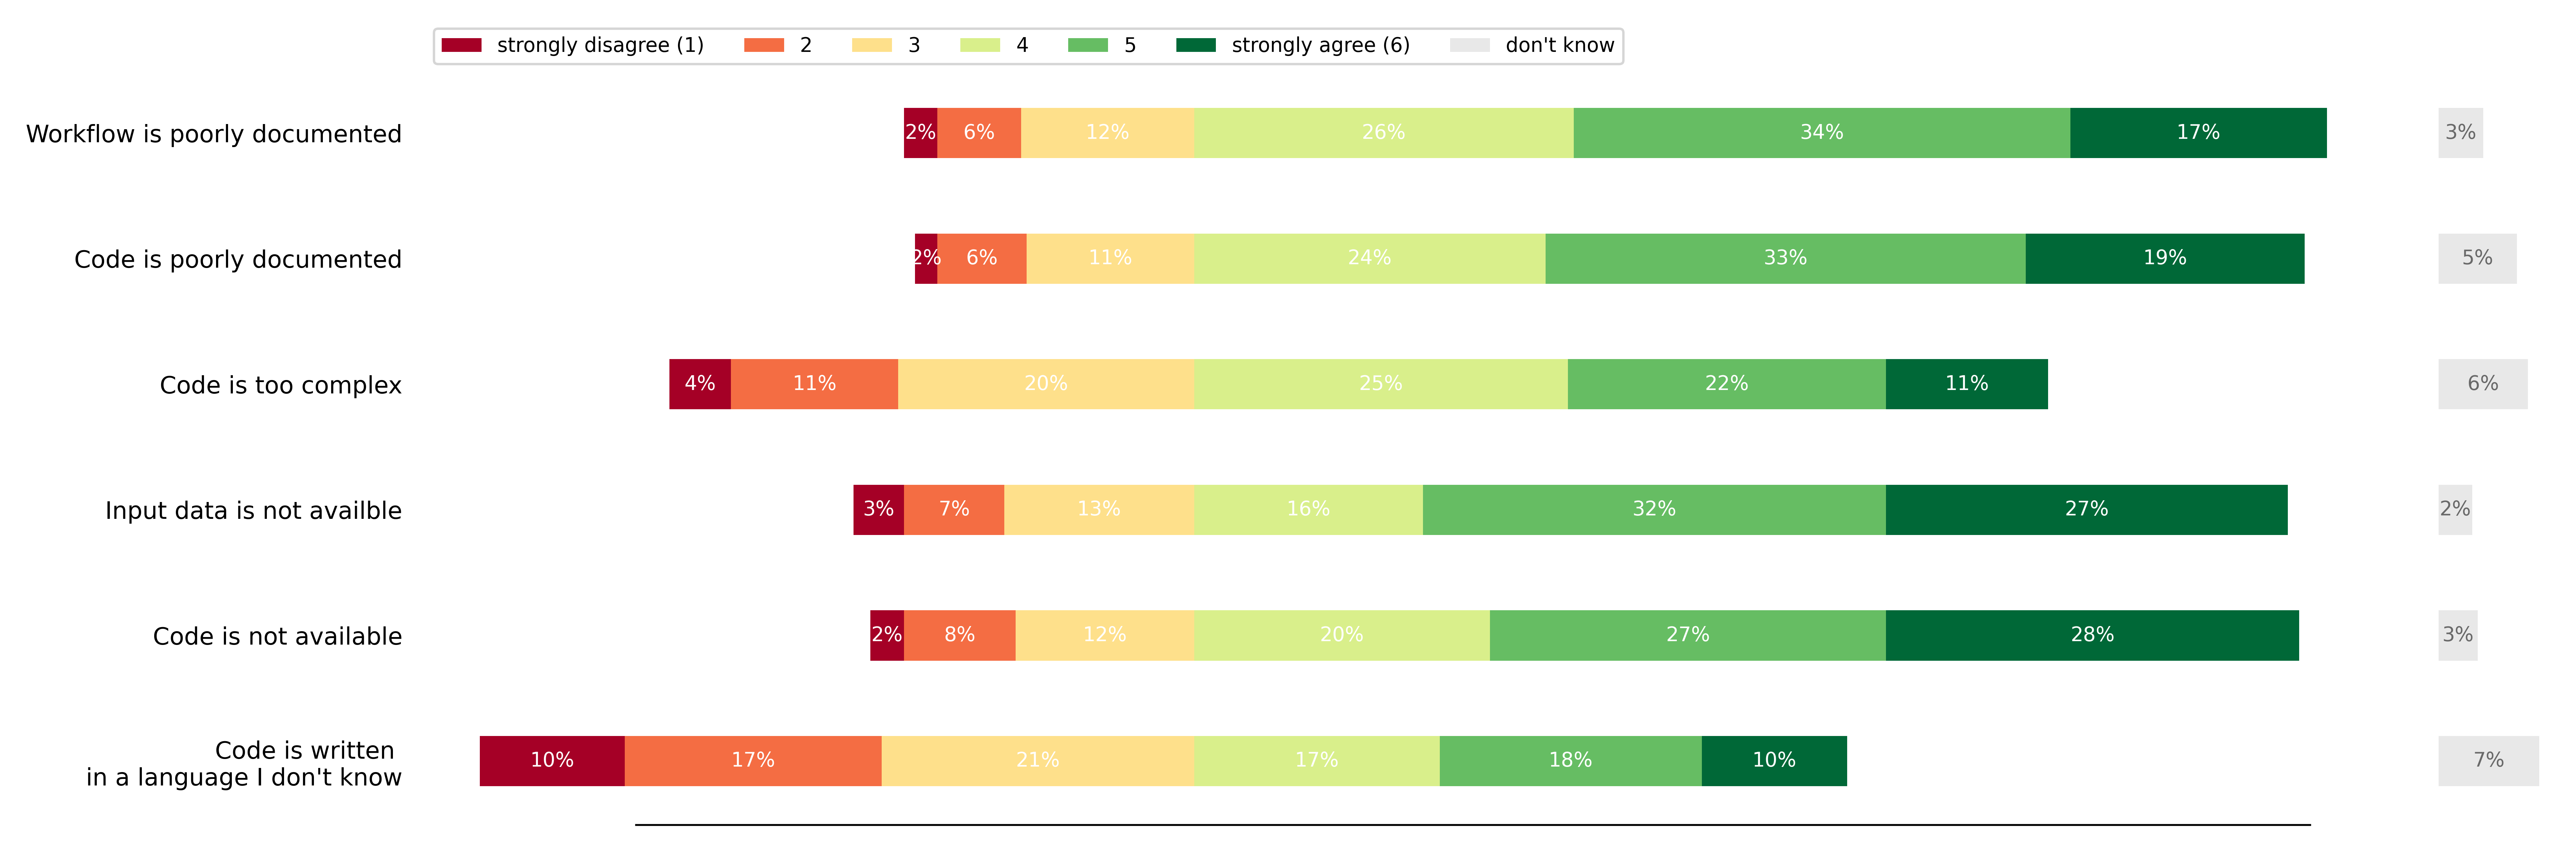
\includegraphics[width=\textwidth]{../figs/O103.png}
	\caption{O103 What are the reasons for poor reproducibility?}
    \label{fig:O103}
\end{figure}

\begin{figure}[!p]
    \centering
    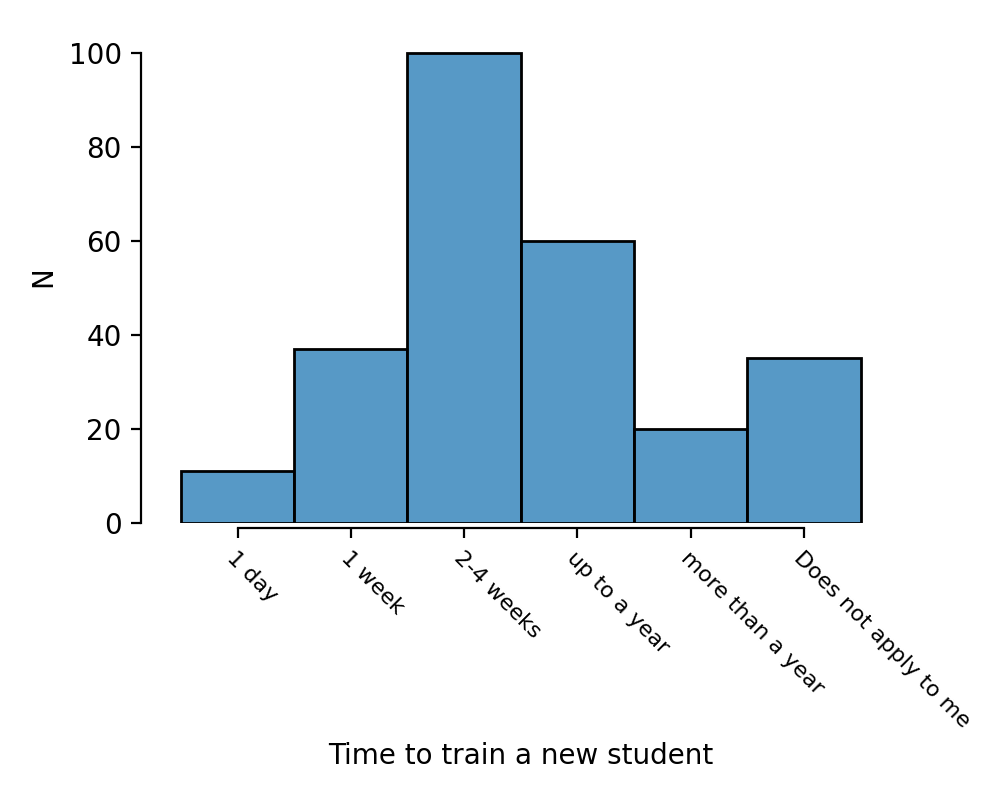
\includegraphics[width=\textwidth]{../figs/S113.png}
	\caption{S113 How long does it take to train a new student in your software?}
    \label{fig:S113}
\end{figure}

\newpage

\subsubsection{H4 Differences in Opinion on Reproducibility}

Number of established (full Prof.) researchers: 32

Number of young (Students, PhD candidates, Postdocs, Junior Prof., Associate Prof.) researchers: 181

Mean agreement to reproducibility: 3.105058

Mean agreement among young sc.: 3.005650

Mean agreement among established sc.: 3.612903

Median agreement to reproducibility: 3.000000

Median agreement among young sc.: 3.000000

Median agreement among established sc.: 4.000000
Career has no normal distribution

No statistical test possible, samples of to low to do a proper Wilcoxon or even t-test


\subsubsection{H5 Reasons for lack of reproducibility}


All answers (without don't know) -  Mean workflow: 4.390438, code documentation : 4.440816, code complexity: 3.884774, input data not available: 4.501976, code availability: 4.500000, written language: 3.473029

Thus, the main reason for a lack of reproducibility is: Input data, then 2: code availability, 3: documentation, 4: workflow, 5: code complexity, 6: language

Mean agreement code complexity 3.884774

Mean agreement among young sc.: 3.784431

Mean agreement among established sc.: 4.033333

Median agreement: 4.000000

Median agreement among young sc.: 4.000000

Median agreement established sc: 4.000000


\subsubsection{H10 Practitioners are less awarte of the issue}

No Data to investiagte this question. Only scientists answered the poll.

\subsubsection{H13 Reasons for reproducibility}

See H5. No addtional data to explore this further.

\subsubsection{H14 Senior researchers are convinced their work is reproducible. (much more at least than young scientists).}


Mean agreement on: my own research is reproducible: 4.428571

Mean agreement among young sc.: 4.413408

Mean agreement among estbalished sc: 4.562500

Median agreement: 5.000000

Median agreement among young sc: 5.000000

Median agreement among established sc.: 5.000000


\subsubsection{H16 Researchers think that their software is bug free and always correspond to their intended implementation.}
We did not ask a question that perfectly relates. Parts are answered in Fig. \ref{fig:O101}.
Main relation to question: Implementing an algorithm based on a description from a publication yourself is the same as using the exact software package/original code that was used in that very publication.


Mean agreement - description is same as implementation: 2.379592


\newpage

\subsection{Reproducibility Practices and Skills}
This part covers "actual" behaviour. (still only self-report assessment, but we can't change that)

    Start here with summary of our hypotheses

We expected to see that... (formulate in a neutral tone)

    Analysis Steps:
        plot corresponding questions (across full sample)
        perform statistical testing of our above stated hypotheses (across subgroups, e.g. early career vs senior researcher)
        perform further data exploration (NOT hypothesis testing) - this might inspire future research, e.g. correlation analysis


Corresponding hypotheses
\begin{itemize}
	\item H6 Researchers code frequently but without knowledge about engeneering methods licences and tools.
	\item H9 Most researchers have never reproduced code with the original model. Only with their own model. This differs between fields.
	\item H12 Most researchers don't know if their software belongs to them.
	\item H2 Young scientists are more familiar with licencing issues.
\end{itemize}



Corresponding survey questions:
\begin{itemize}
	\item O102 Did you actively reproduce scientific results in the past?
	\item S103 How often do you use research software?
	\item S110 How often do you develope research software?
	\item S202 Do you own your software?
	\item S112 Which licences are familiar?
	\item S101 What kind of programming languages are used?
	\item S111 Which licences do you use?
	\item S104 Do you practice any of the following methods?
	\item S105 Do you these tools?
	\item S106 Gow did you learn to program?
\end{itemize}

\begin{figure}[!p]
    \centering
    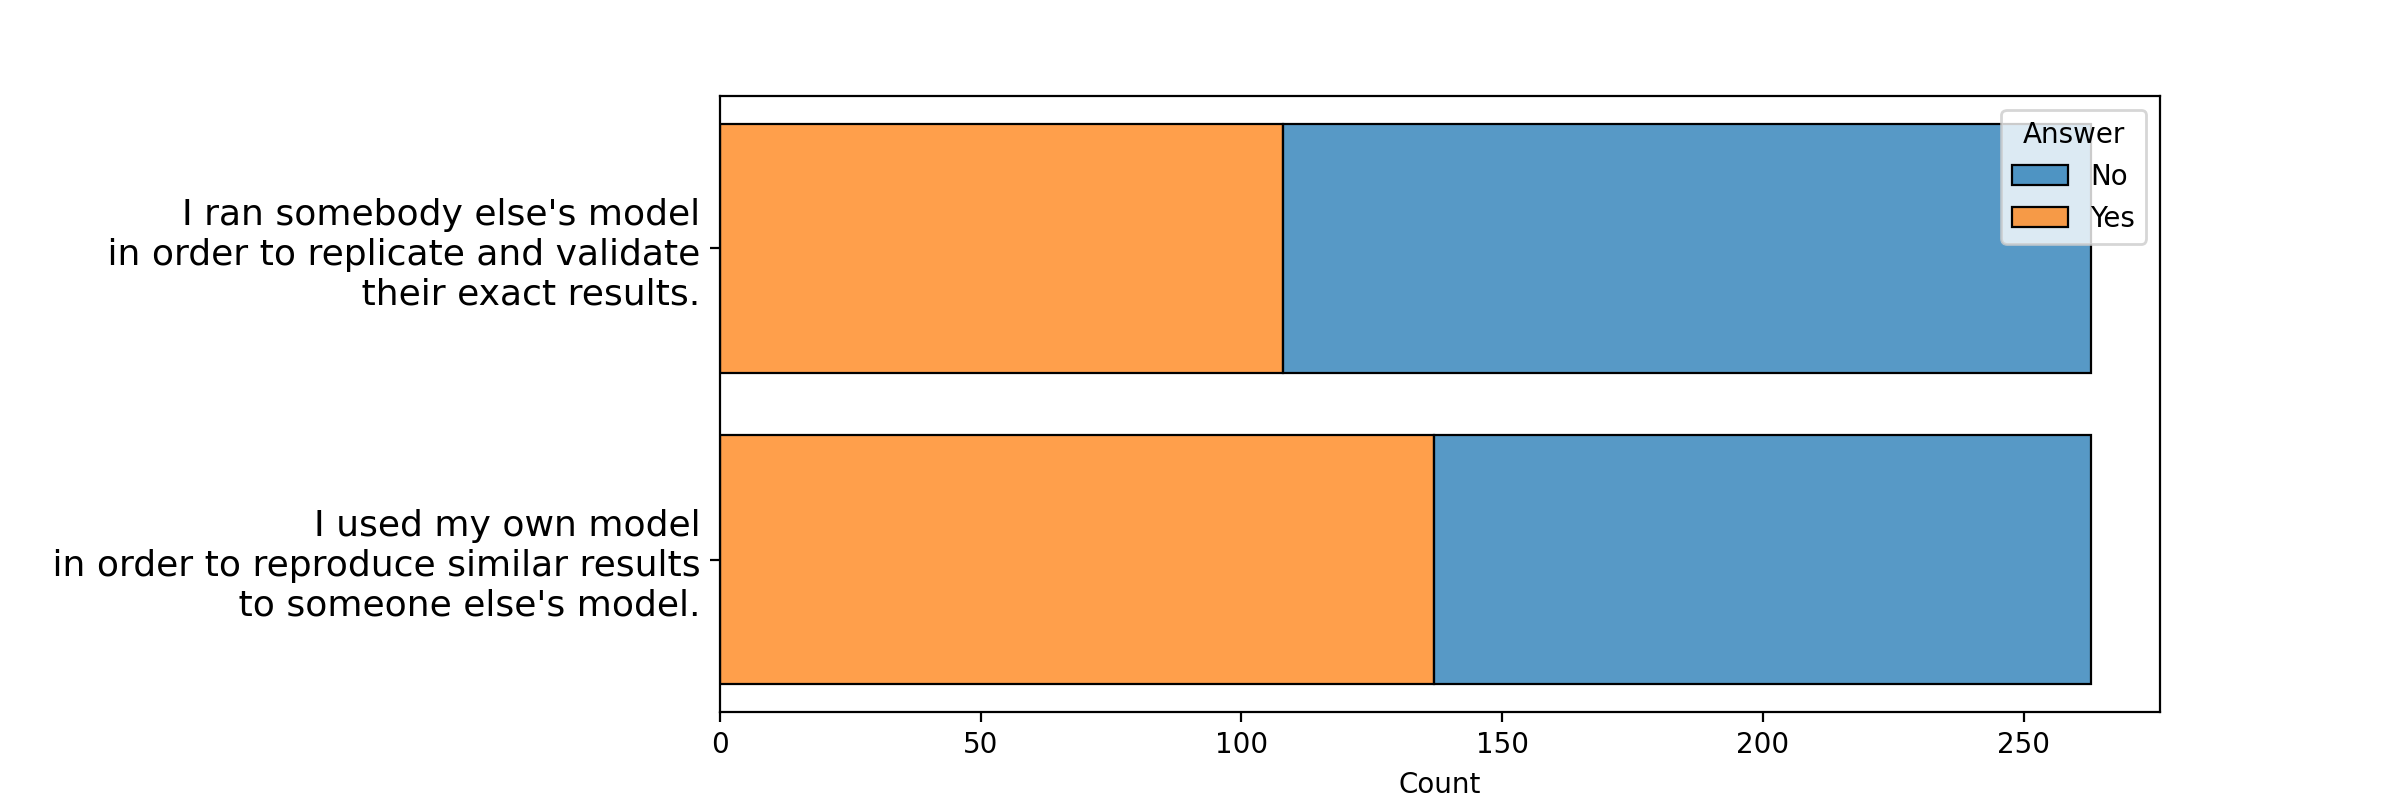
\includegraphics[width=\textwidth]{../figs/O102.png}
	\caption{O102 Did you reproduce results?}
    \label{fig:O102}
\end{figure}

\begin{figure}[!p]
    \centering
    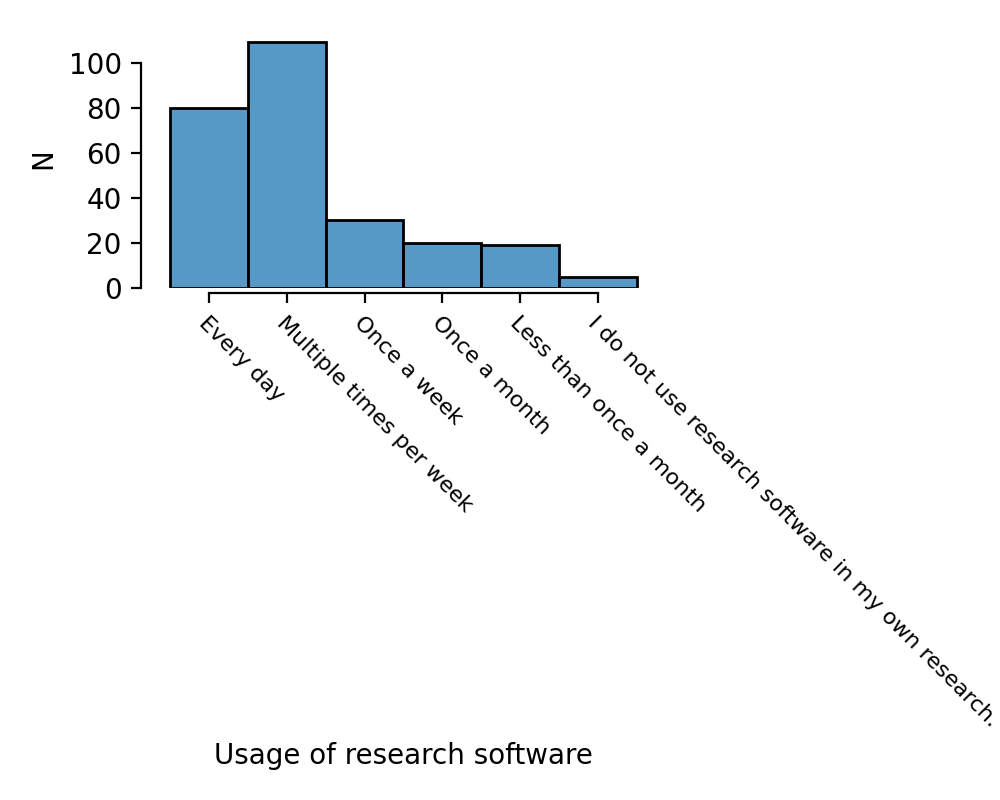
\includegraphics[width=\textwidth]{../figs/S103.png}
	\caption{S103 Frequence of using software.}
    \label{fig:S103}
\end{figure}

\begin{figure}[!p]
    \centering
    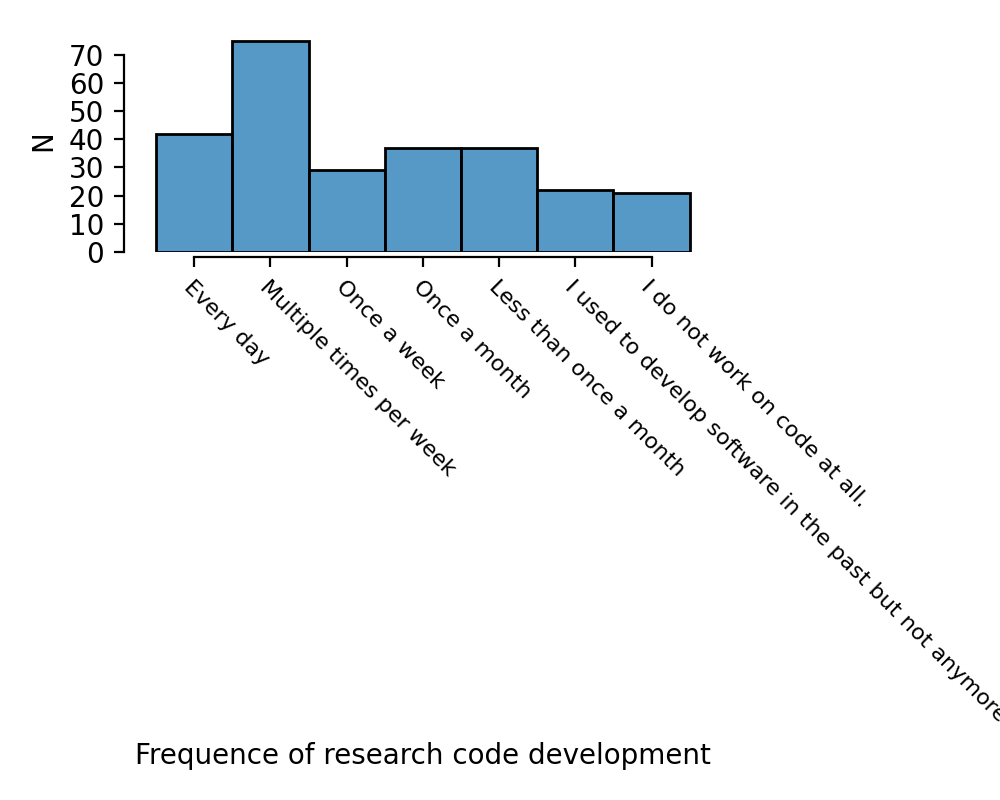
\includegraphics[width=\textwidth]{../figs/S110.png}
	\caption{S110 Frequence of developing software}
    \label{fig:S110}
\end{figure}

\begin{figure}[!p]
    \centering
    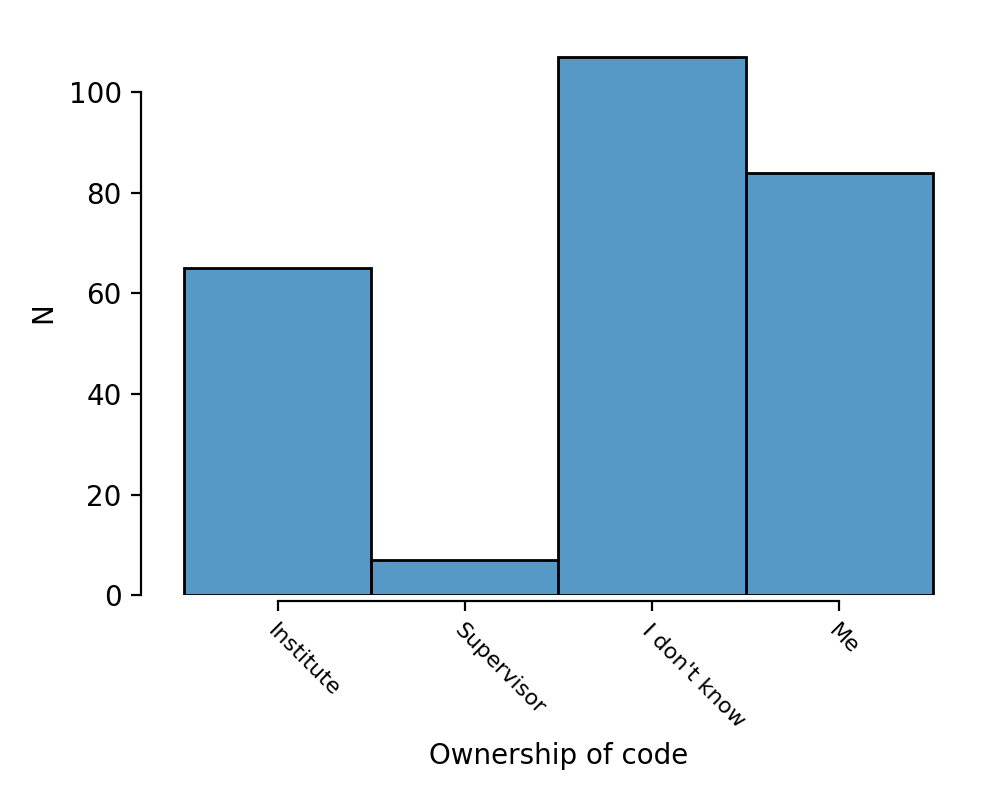
\includegraphics[width=\textwidth]{../figs/S202.png}
	\caption{S202 Do you own your software?}
    \label{fig:S202}
\end{figure}

%\include{S112.tex}
%\include{S101.tex}
%\include{S111.tex}
%\include{S104.tex}
%\include{S105.tex}
%\include{S106.tex}

\subsubsection{H9 Activity of reproduction}

\textbf{XX}

\subsection{Hurdles against and Solutions towards Reproducibility}

This part covers "actual" behaviour. (still only self-report assessment, but we can't change that)

    Start here with summary of our hypotheses

We stated that... (formulate in a neutral tone)

    Analysis Steps:
        plot corresponding questions (across full sample)
        perform statistical testing of our above stated hypotheses (across subgroups, e.g. early career vs senior researcher)
        perform further data exploration (NOT hypothesis testing) - this might inspire future research, e.g. correlation analysis

    corresponding hypotheses (see Robert's evaluation plan):
        H7
        H13
        H3

    Corresponding survey questions:
        S203 - What keeps you from publishing as open source?
        S201 - What would help to increase reproducibility?
        S204 (open text)

\begin{figure}[!p]
    \centering
    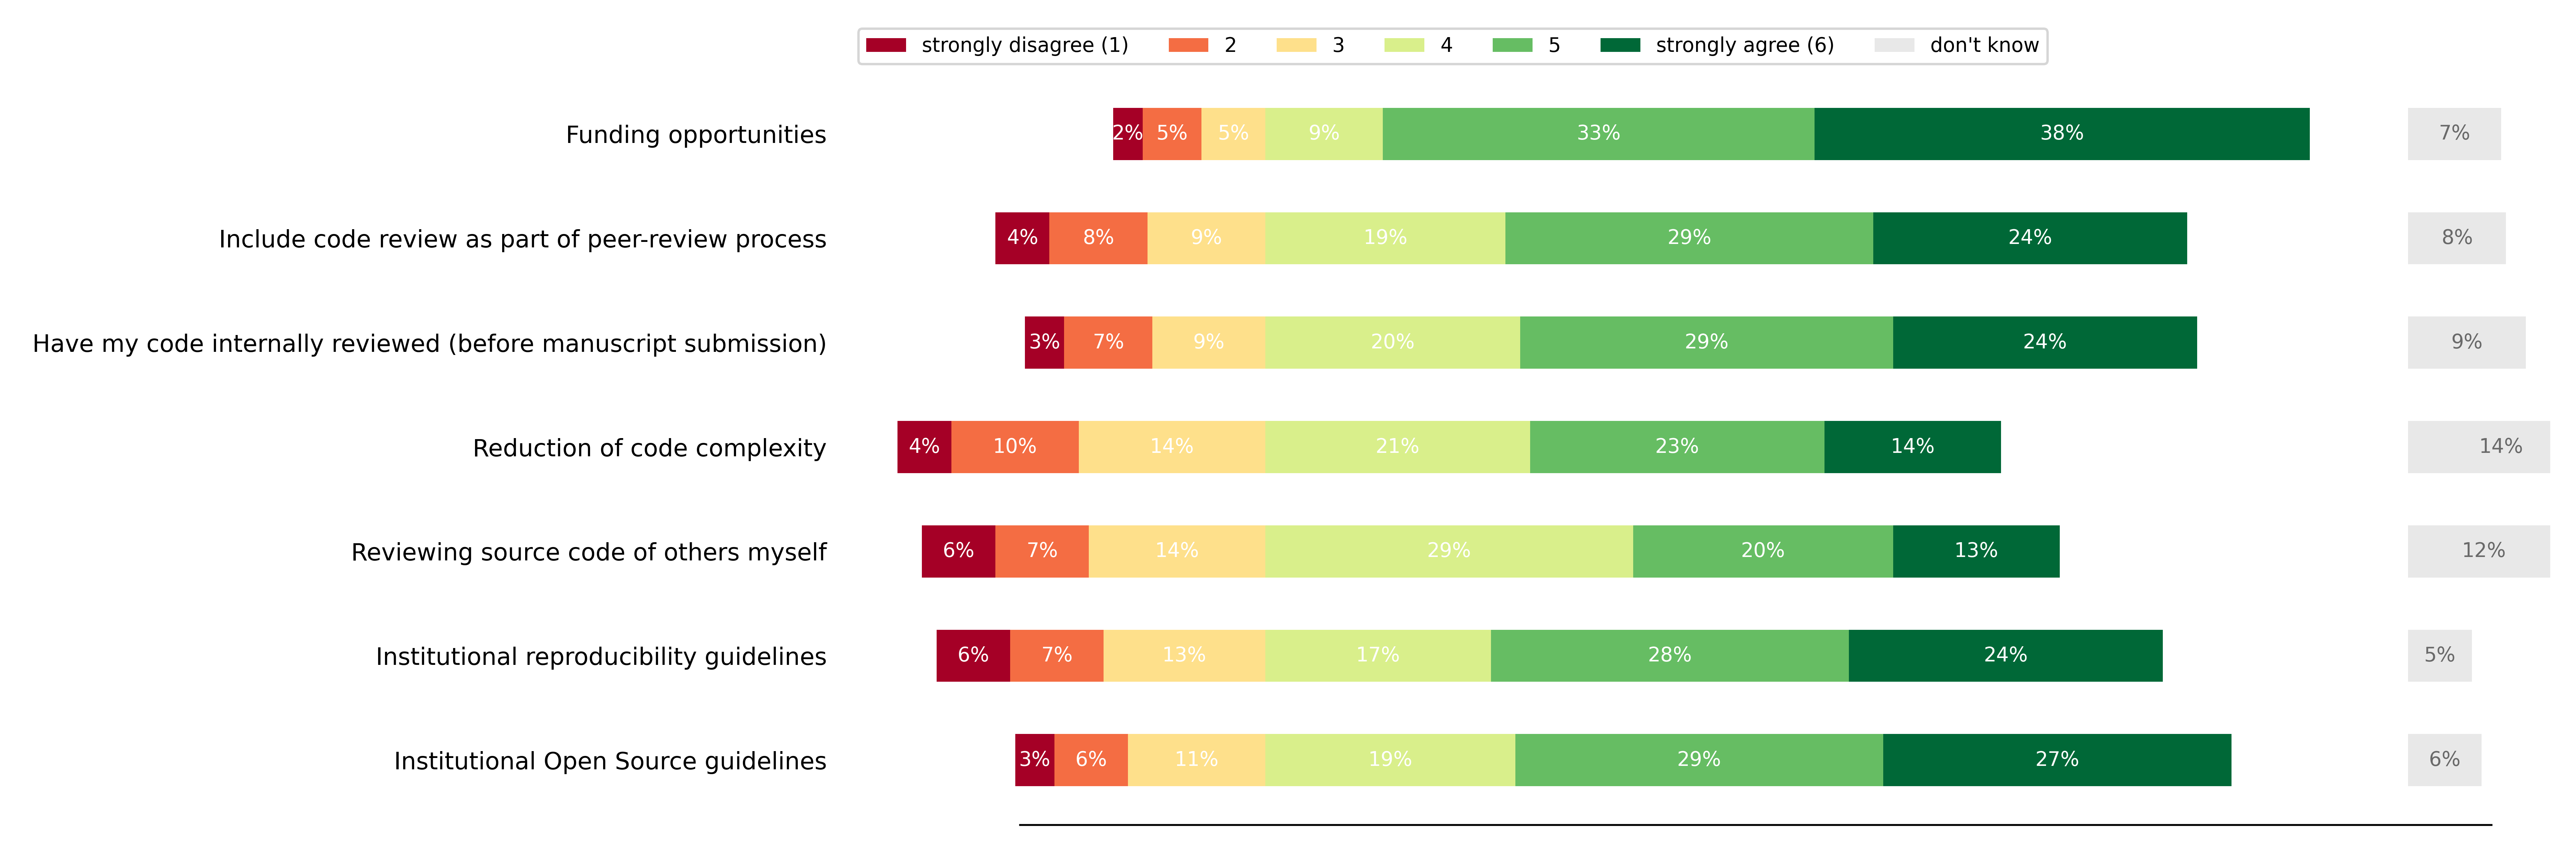
\includegraphics[width=\textwidth]{../figs/S201.png}
	\caption{S201 }
    \label{fig:S201}
\end{figure}

\begin{figure}[!p]
    \centering
    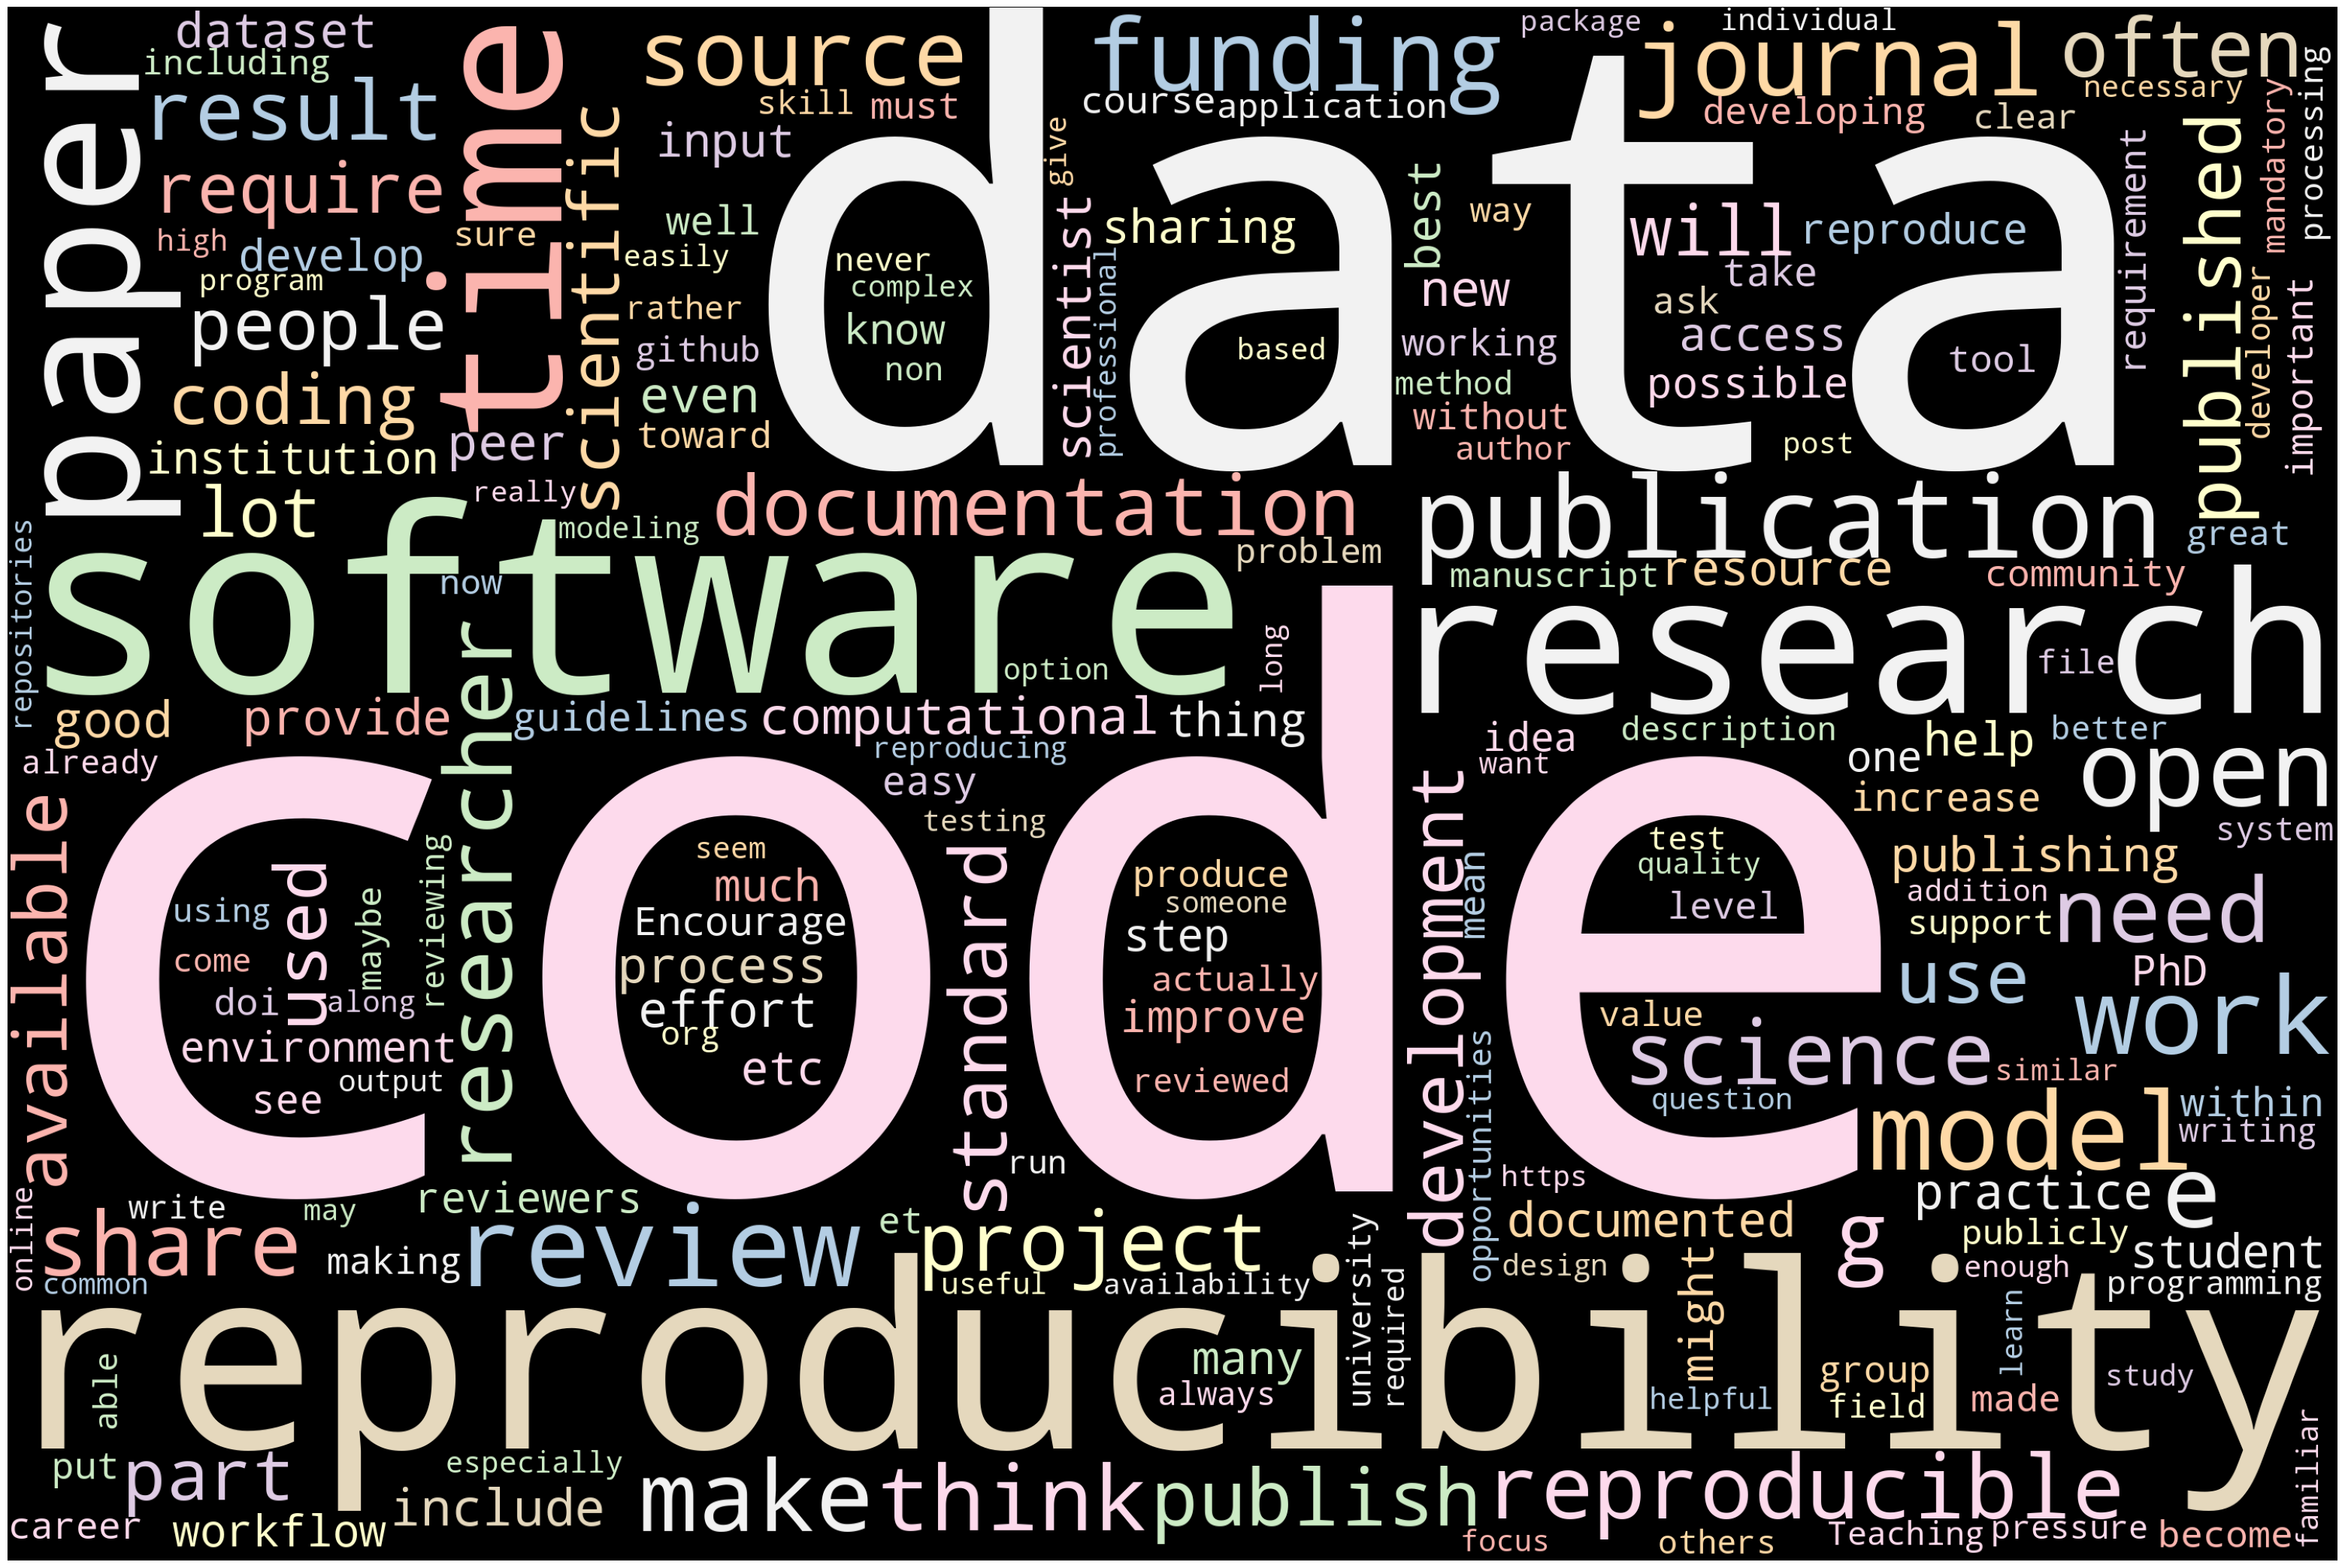
\includegraphics[width=\textwidth]{../word_cloud.png}
	\caption{Full text answers as word cloud }
    \label{fig:wc}
\end{figure}

\end{document}
